\clearpage
\section{MET disagreement investigation}
\label{MET_disagreement_investigation}

***NOTE: The following mitigation method for Data/MC disagreement is not applied to the analysis anymore.

%In step 2, we use MET cuts to suppress DY contribution in same flavor channel. Therefore, we should make sure that MC simulation is able to describe data reasonably.
The MET agreement between data and MC is not good which can be seen in
Figure \ref{fig:step1_MET_phi}.
The problem is present in same flavor channel mostly from DY process which has not real MET.

\subsubsection {Source of MET disagreement}
Due to the fact that there is no real MET (comes from neutrino in W decay) in DY process and MET in this process originate from jets, we conclude that the problem can come from the following sources.

$\bullet$ modeling of the vector-boson recoil and detector effects, which can be difficult to simulate accurately and deficiencies in the modeling of the calorimeter response and resolution \cite{recoil}
%$\bullet$ incomplete description of the underlying event.

$\bullet$ poor simulation of number of pile up

In order to investigate the simulation of recoiled jet, we looked at the  $|\Delta \phi|$ between MET and dilepton.
We expect to see MET disagreement, because of the poor simulation of the recoiled jets, mostly  close to 0 or $\pi$.
In Figure \ref{fig:step1_H_MET_Z_T1Txy_phi}, the distribution of $|\Delta \phi|$(MET,ll) is shown. We see disagreement close to the $\pi$.
So if the source of MET disagreement is related to the events with a high \pt jet recoiling against jet, we should see good agreement for events without such a jet.
We put a cut on $|\Delta \phi|$(MET,ll)$<$2 and looked at MET distribution which can be seen in Figure \ref{fig:step1_H_MET_Z_T1Txy_phi}.
It can be seen that MET has similar shape and the disagreement source is not the poor simulation of recoiled jet.


As it can be seen in Figure \ref{fig:step1_pv_n}, the distribution of number of reconstructed vertices is different for data and MC and pileup reweighting does not work properly.
Due to the fact that there is a correlation between MET and number of pileup, disagreement in number of vertex distribution can be propagated into the MET distribution.
In Figure \ref{fig:step1_MET_Nvtx},  MET distributions are shown for events with number
of vertices in various bins  after step1 selection. One can see that the ratio of data and MC for the MET (MET shape) is
much more flat compare with the nominal plot (see figure
\ref{fig:step1_MET_phi}) although the ratio of data MC normalization is not 1 because of the fact that pile-up
reweighting does not work well. After finding the relation between MET and number
of vertices, we do a reweighting using number of vertices in same flavor channels. The results
are shown in Figure \ref{fig:step1_Nvtx_reweight}. The data MC agreement has improved clearly.

\begin{figure}[ht]
  \begin{center}
    \begin{tabular}{ccc}
      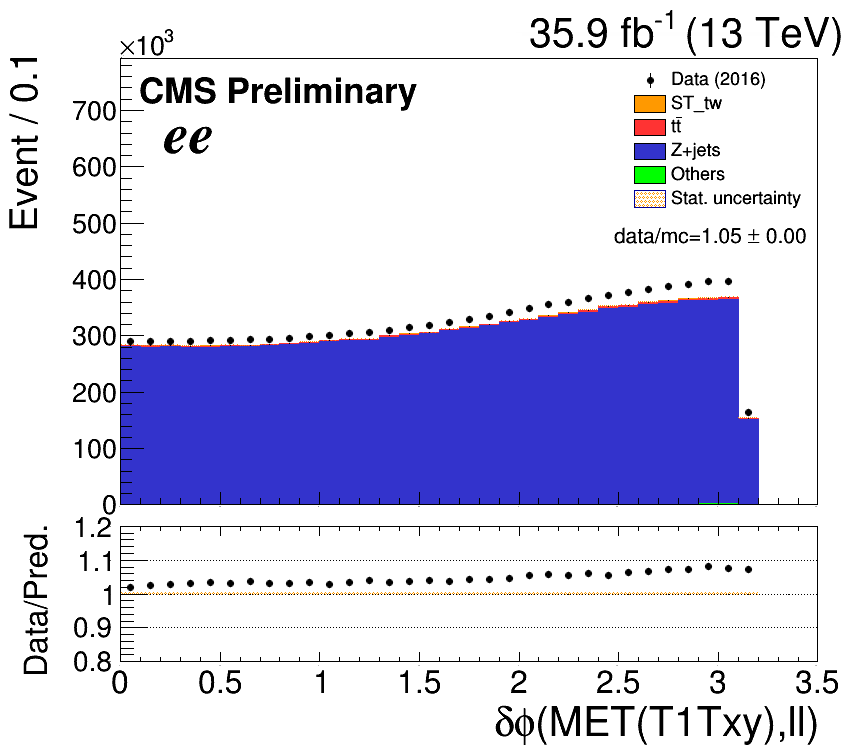
\includegraphics[width=0.4\textwidth]{figures/tW/fig/Step1/ee_noNvtx/H_MET_Z_T1Txy_phi.png}&
      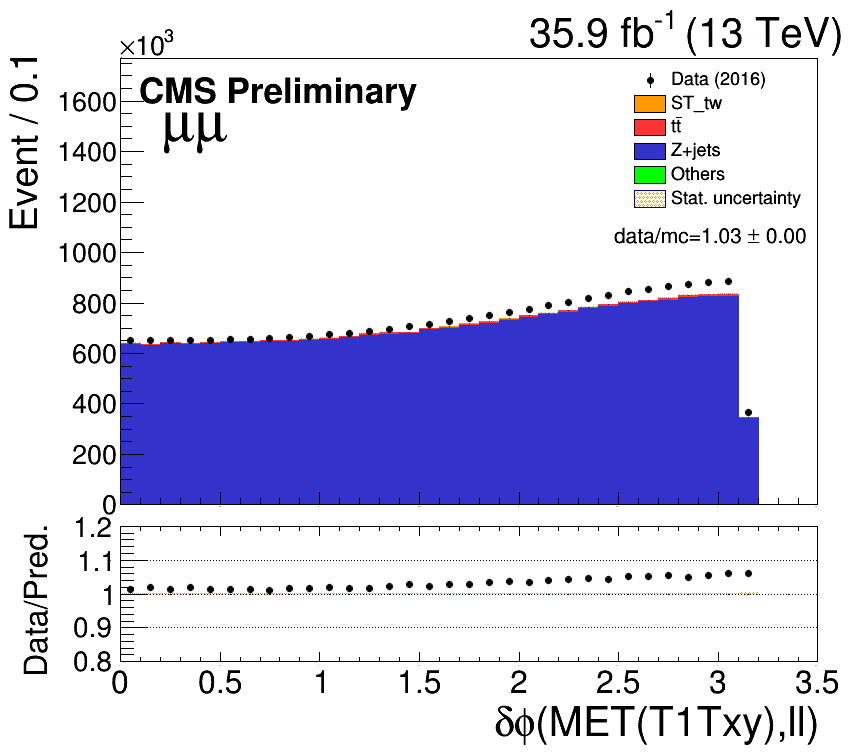
\includegraphics[width=0.4\textwidth]{figures/tW/fig/Step1/mumu_noNvtx/H_MET_Z_T1Txy_phi.png}\\
      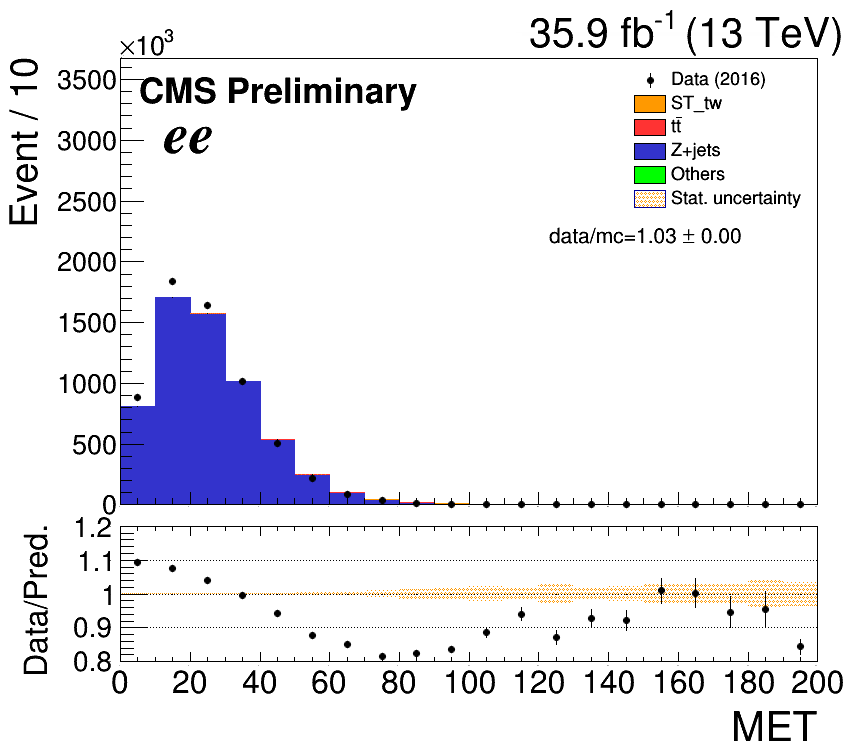
\includegraphics[width=0.4\textwidth]{figures/tW/fig/ee_H_MET_Et.png}&
      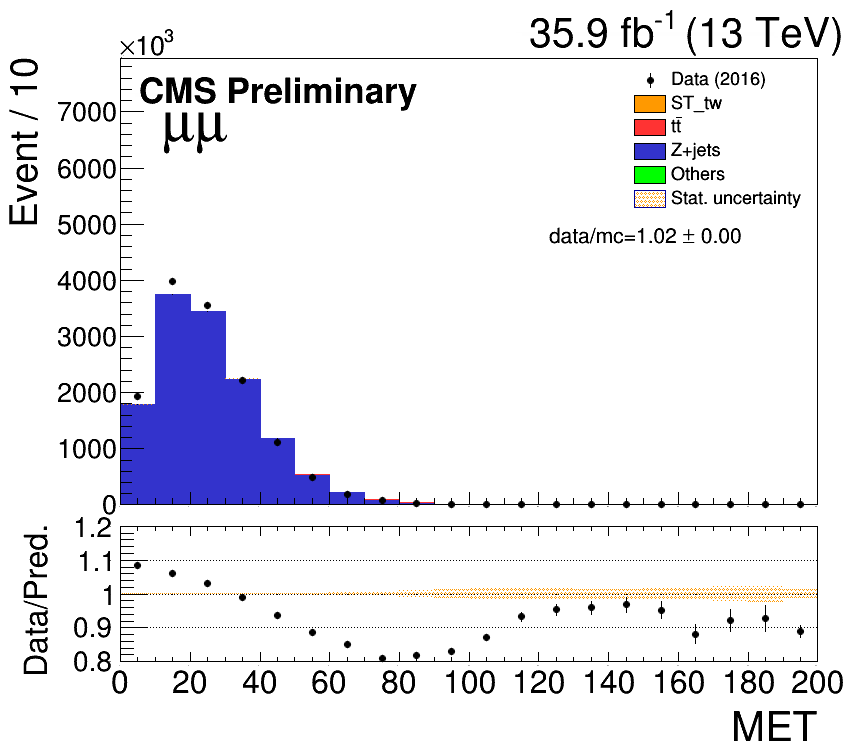
\includegraphics[width=0.4\textwidth]{figures/tW/fig/mumu_H_MET_Et.png}\\
    \end{tabular}
    \caption{The distributions of the $\Delta \phi$ (MET,ll) (first row), MET (second row) for events with $\Delta \phi$ (MET,ll)<2, for ee (left) and \mumu (right) channels after step 1.
    \label{fig:step1_H_MET_Z_T1Txy_phi}}
  \end{center}
\end{figure}

\begin{figure}[ht]
  \begin{center}
    \begin{tabular}{ccc}
      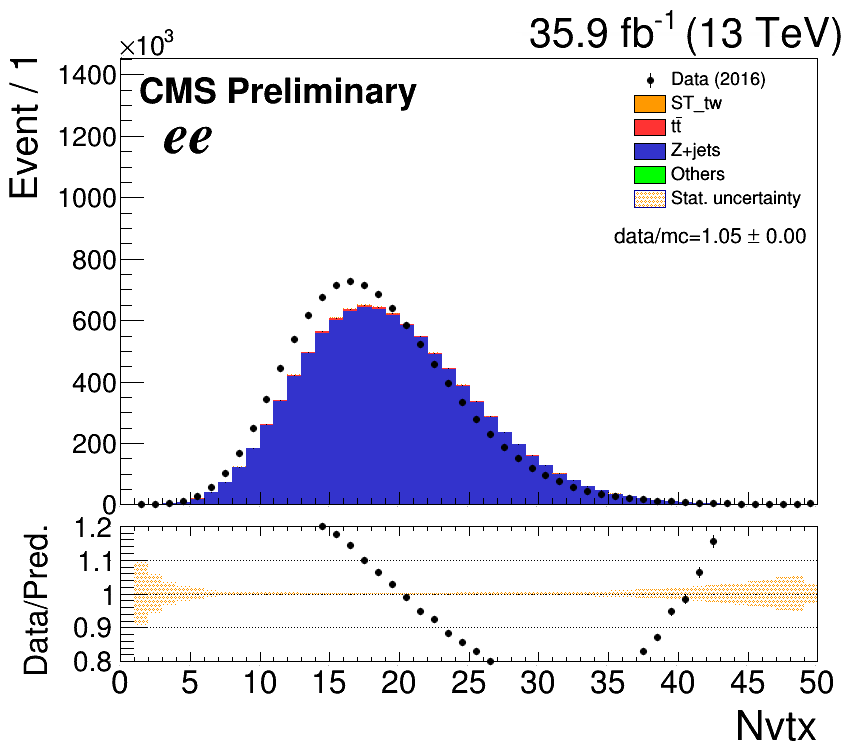
\includegraphics[width=0.4\textwidth]{figures/tW/fig/Step1/ee_noNvtx/H_pv_n.png}
      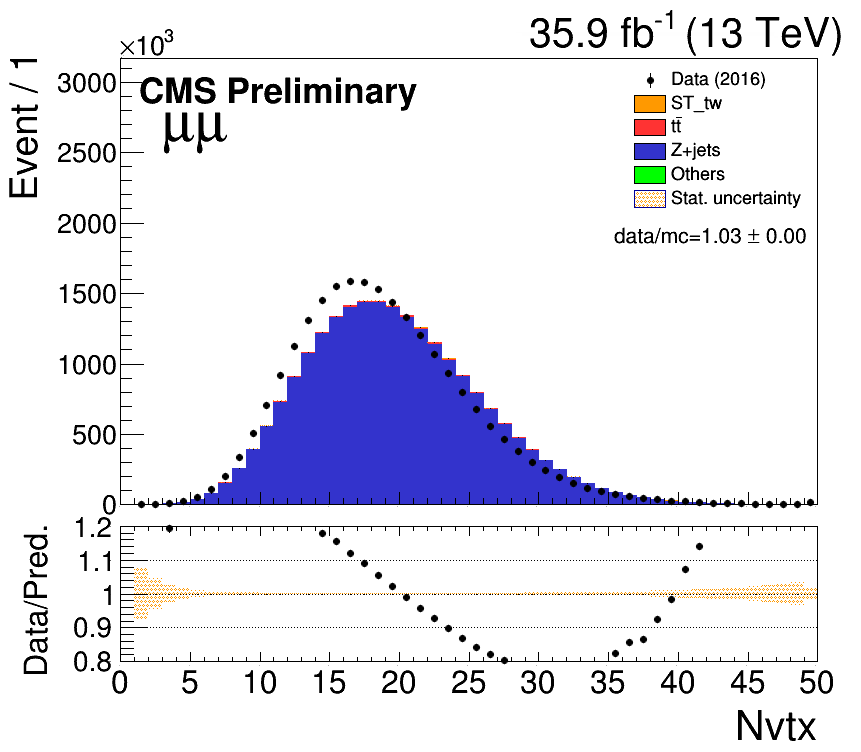
\includegraphics[width=0.4\textwidth]{figures/tW/fig/Step1/mumu_noNvtx/H_pv_n.png}
    \end{tabular}
    \caption{The distributions of number of reconstructed vertices for ee (left) and \mumu (right) channels after step 1.
    \label{fig:step1_pv_n}}
  \end{center}
\end{figure}



\begin{figure}[ht]
  \begin{center}
    \begin{tabular}{ccc}
      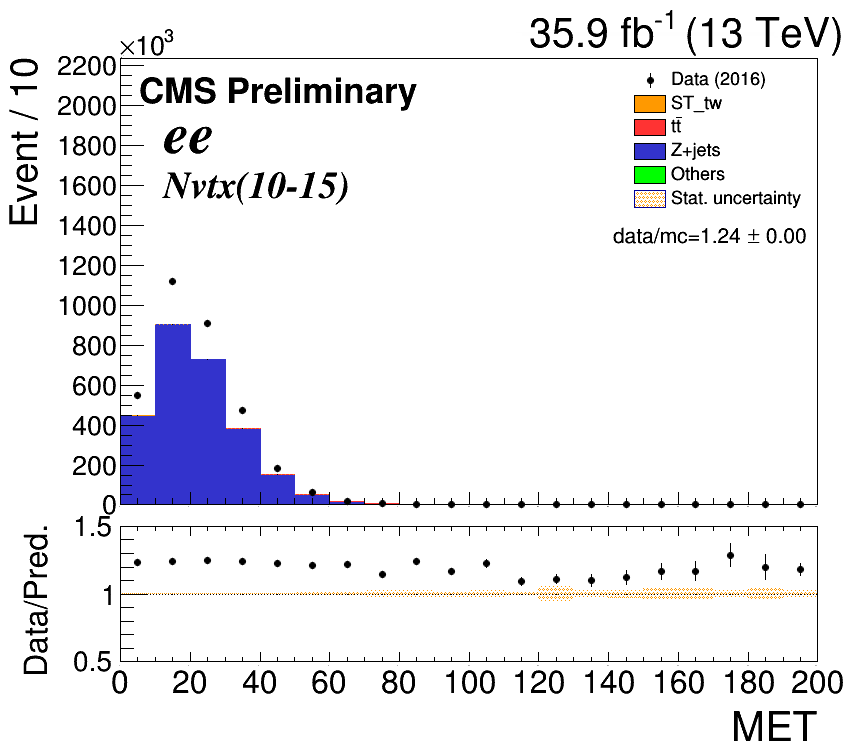
\includegraphics[width=0.4\textwidth]{figures/tW/fig/Nvtx/10-15/ee/H_MET_Et.png}&
      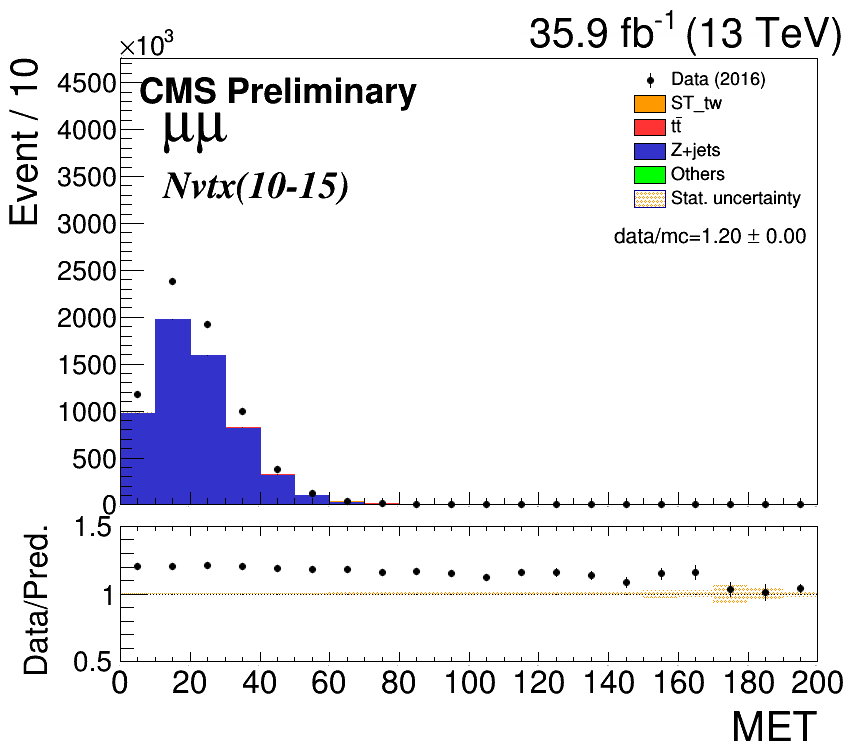
\includegraphics[width=0.4\textwidth]{figures/tW/fig/Nvtx/10-15/mumu/H_MET_Et.png}\\
      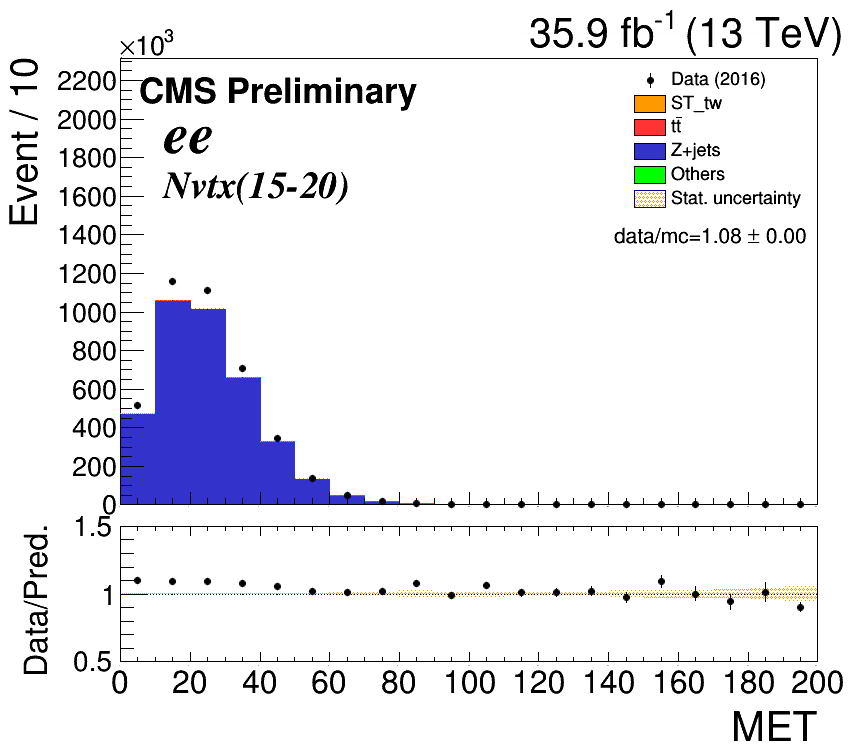
\includegraphics[width=0.4\textwidth]{figures/tW/fig/Nvtx/15-20/ee/H_MET_Et.png}&
      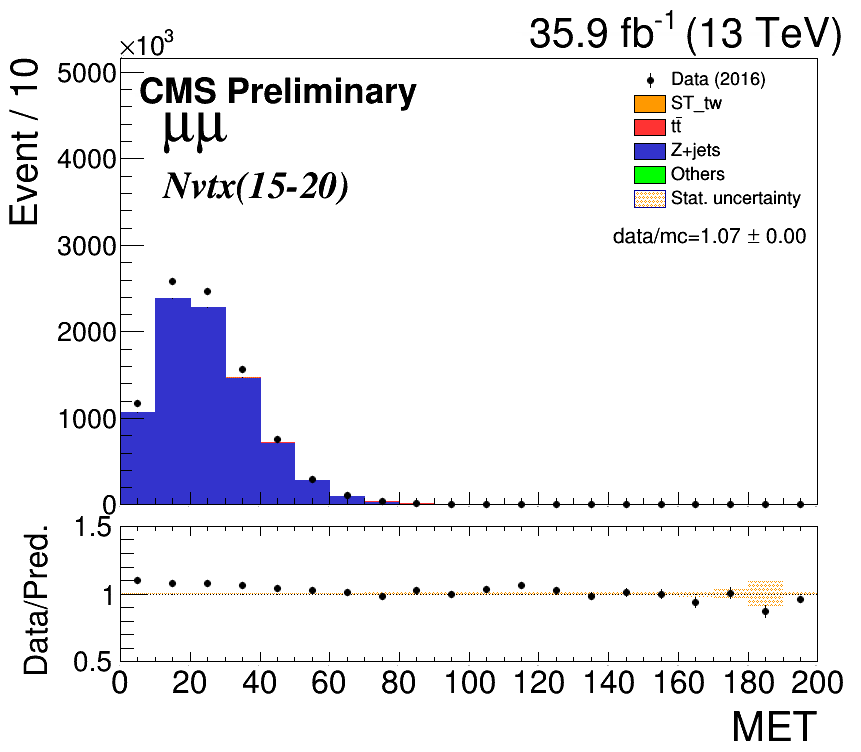
\includegraphics[width=0.4\textwidth]{figures/tW/fig/Nvtx/15-20/mumu/H_MET_Et.png}\\
      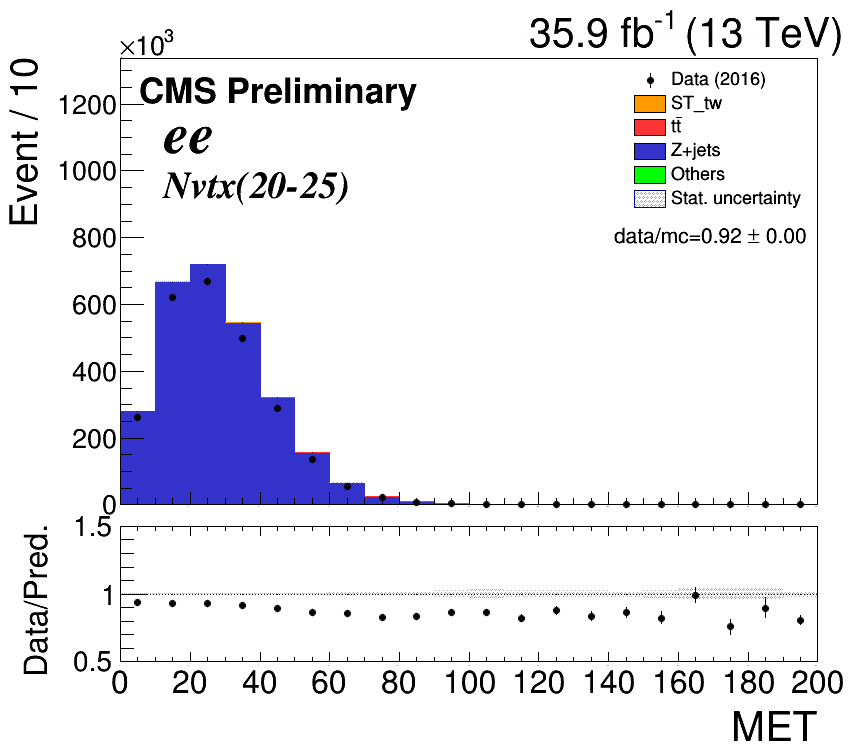
\includegraphics[width=0.4\textwidth]{figures/tW/fig/Nvtx/20-25/ee/H_MET_Et.png}&
      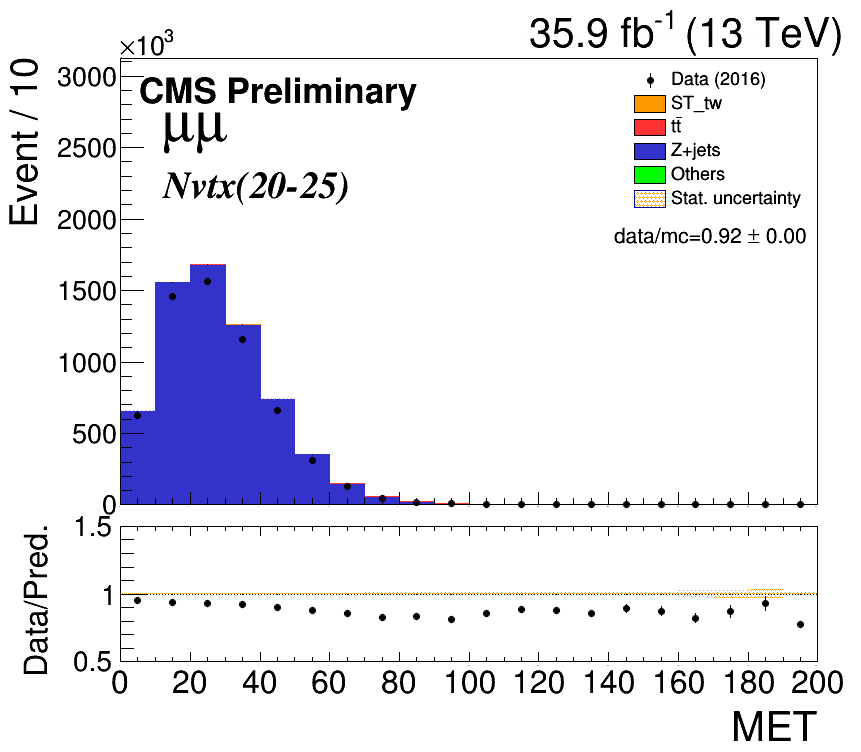
\includegraphics[width=0.4\textwidth]{figures/tW/fig/Nvtx/20-25/mumu/H_MET_Et.png}\\
      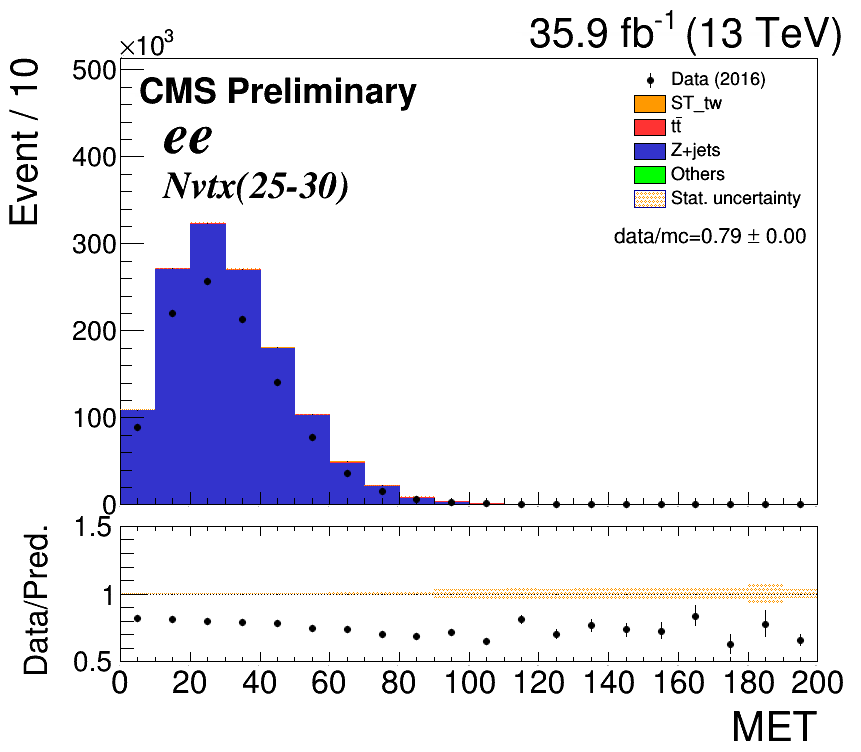
\includegraphics[width=0.4\textwidth]{figures/tW/fig/Nvtx/25-30/ee/H_MET_Et.png}&
      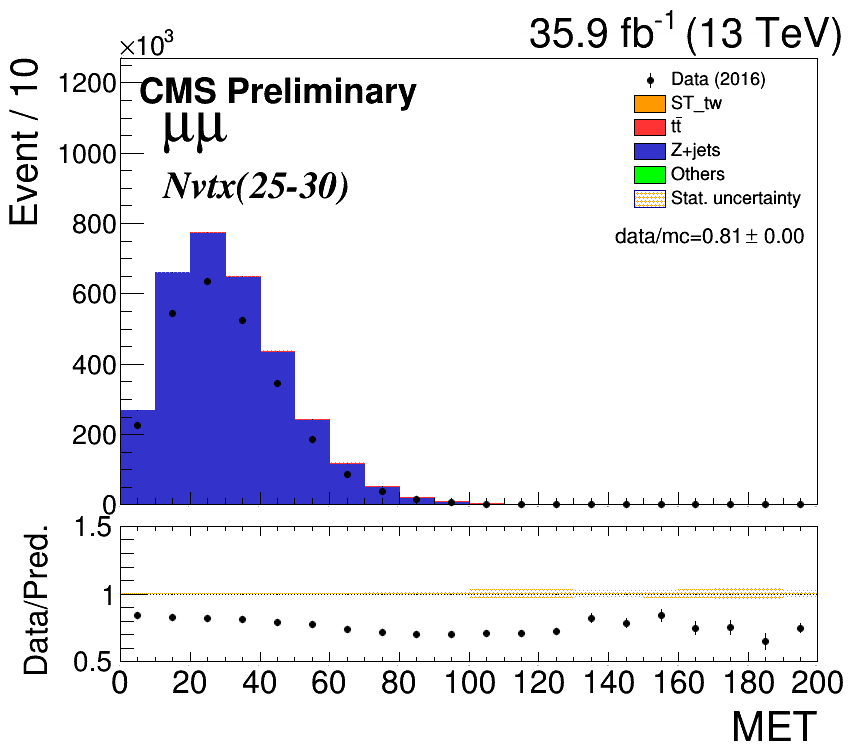
\includegraphics[width=0.4\textwidth]{figures/tW/fig/Nvtx/25-30/mumu/H_MET_Et.png}\\
    \end{tabular}
    \caption{The distributions of MET for events with number of vertices between 10-15 (first row), 15-20 (second row), 20-25 (third row) and 25-30 (last row) for ee (left) and \mumu (right) channels.
    \label{fig:step1_MET_Nvtx}}
  \end{center}
\end{figure}


\begin{figure}[ht]
  \begin{center}
    \begin{tabular}{ccc}
      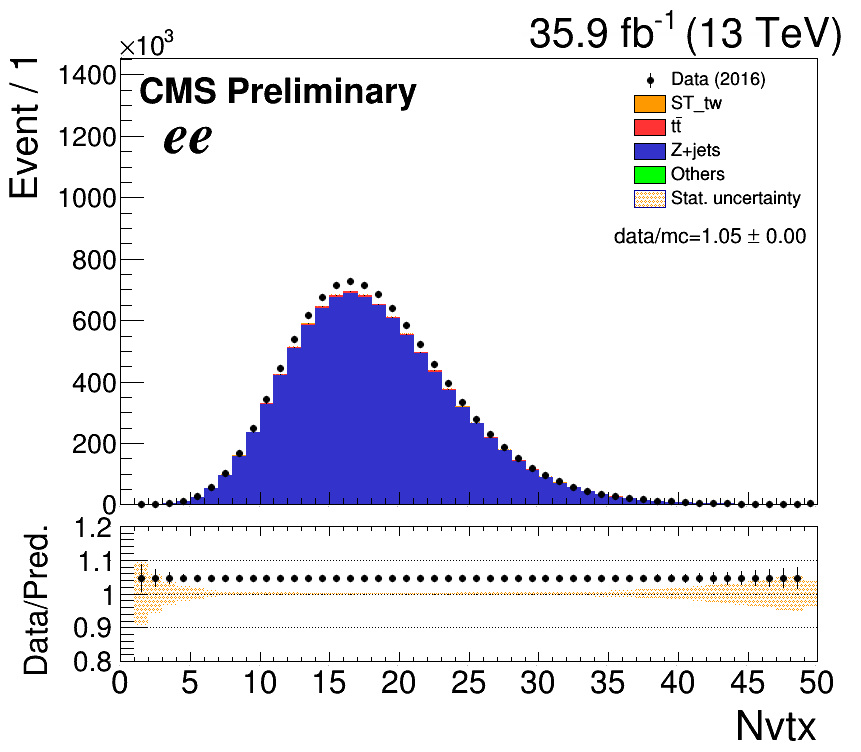
\includegraphics[width=0.4\textwidth]{figures/tW/fig/Step1/ee_Nvtx/H_pv_n.png}&
      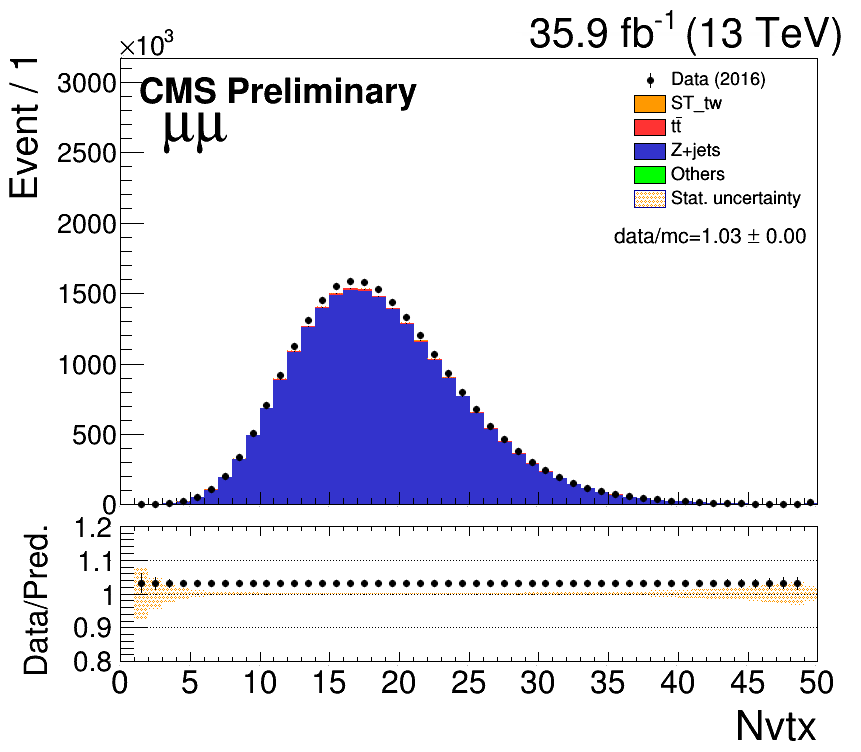
\includegraphics[width=0.4\textwidth]{figures/tW/fig/Step1/mumu_Nvtx/H_pv_n.png}\\
      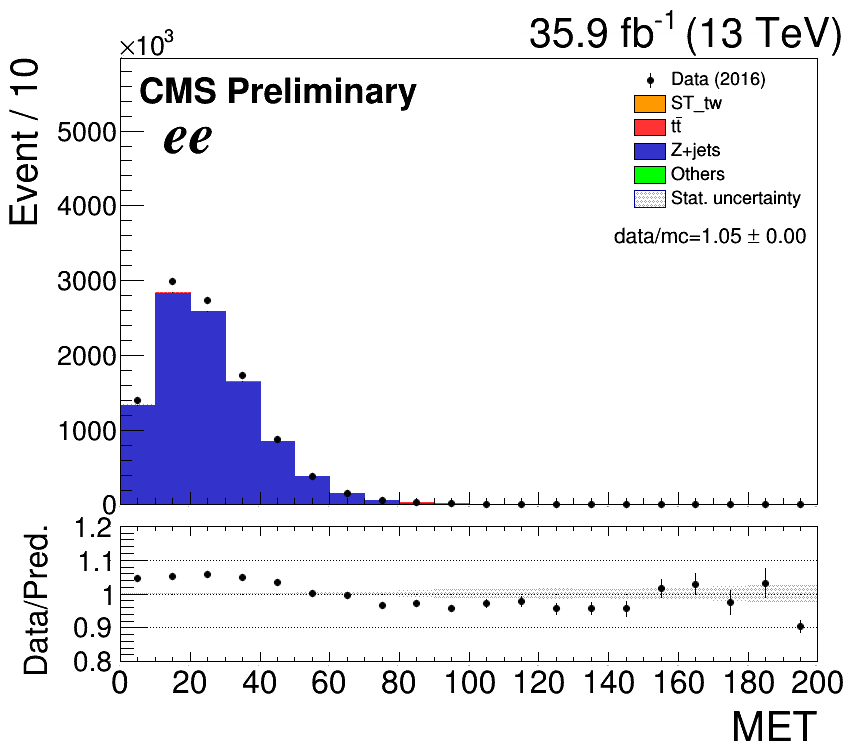
\includegraphics[width=0.4\textwidth]{figures/tW/fig/Step1/ee_Nvtx/H_MET_Et.png}&
      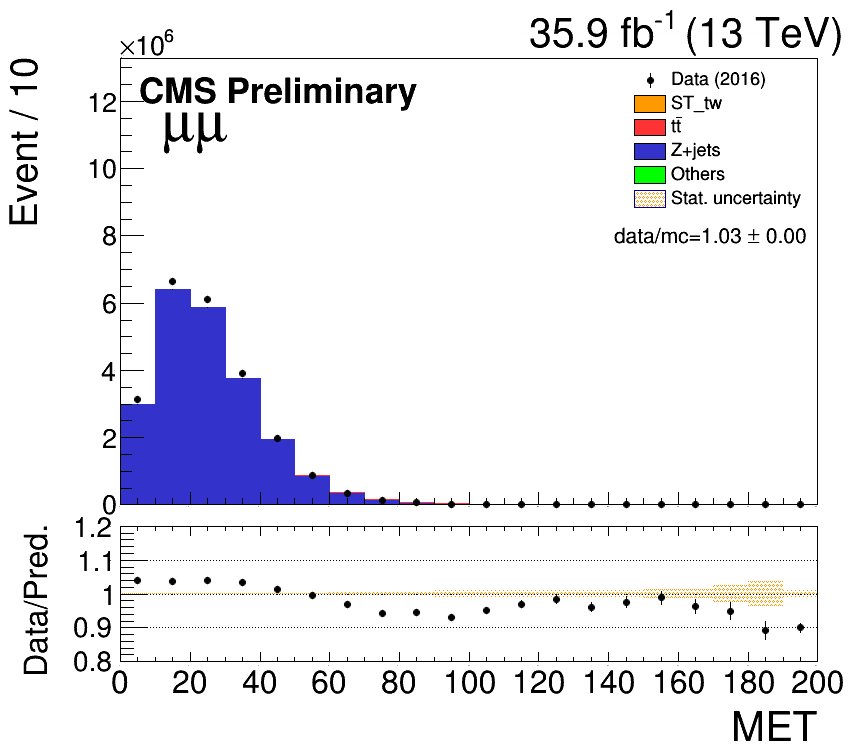
\includegraphics[width=0.4\textwidth]{figures/tW/fig/Step1/mumu_Nvtx/H_MET_Et.png}\\
    \end{tabular}
    \caption{The distributions of number of vertices (top) and MET (bottom) after number of vertices re-weighting for ee (left) and \mumu (right) channels.
    \label{fig:step1_Nvtx_reweight}}
  \end{center}
\end{figure}


